%~~~~~~~~~~~~~~~~~~~~~~~~~~~~~~~~~~~~~~~~~~~~~~~~~~~~~~~~~~~~~~~~~~~~~~~~~~~~~~~~~~~~~~~~~
% Official IISER Thiruvananthapuram Thesis/Dissertation Format
% LaTeX Template for Overleaf
%
% Copyright (c) 2022 by Nikhil Alex
%
% Licensed under Creative Commons Attribution–NonCommercial–ShareAlike 4.0
% (CC BY-NC-SA 4.0). More info: https://creativecommons.org/licenses/by-nc-sa/4.0/
%
% Suggestions/Feedback: nikhil.alexv17@alumni.iisertvm.ac.in
%~~~~~~~~~~~~~~~~~~~~~~~~~~~~~~~~~~~~~~~~~~~~~~~~~~~~~~~~~~~~~~~~~~~~~~~~~~~~~~~~~~~~~~~~~

% Comments like this begin with a % character. 
% Ctrl+b for \textbf{bold} and Ctrl+i for \textit{italics} 
% Ctrl+/ to comment out lines

%=========================================================================================
% PREAMBLE (PACKAGES AND DOCUMENT CONFIGURATION)
%=========================================================================================

% Rewrite the input fields marked with [] brackets.
% Read all uncommented lines carefully.

%~~~~~~~~~~~~~~~~~~~~~~~~~~~~~~~~~~~~~~~~~~~~~~~~~~~~~~~~~~~~~~~~~~~~~~~~~~~~~~~~~~~~~~~~~

\documentclass[12pt,oneside,a4paper]{report} % Font size (pt)
% Add in draft parameter to hide non-essential elements for faster compile times

% Load configuration files
%=========================================================================================
% PACKAGES — ORGANIZED BY CATEGORY
%=========================================================================================

%-----------------------------------------------------------------------------------------
% MATH & SYMBOLS
%-----------------------------------------------------------------------------------------

\usepackage{amsmath}       % Core AMS math features
\usepackage{amsfonts}      % Math fonts
\usepackage{amssymb}       % Extended math symbols
\usepackage{amsthm}        % Theorem and proof environments
\usepackage{mathrsfs}      % Script-style math fonts
\usepackage{yhmath}        % Wide accents
\usepackage{empheq}        % Highlight/emphasise equations
\usepackage{bm}            % Bold math symbols
\usepackage{mathtools}     % Enhancements to amsmath
\usepackage{nccmath}       % Compact math environments 
\usepackage{subcaption}
\usepackage{multicol}
%-----------------------------------------------------------------------------------------
% DOCUMENT LAYOUT
%-----------------------------------------------------------------------------------------

\usepackage{setspace}      % Line spacing control
\usepackage{geometry}      % Page size and margin settings
\geometry{
    a4paper,               % Paper size
    centering,
    left=0.75in,           % Margins
    right=0.75in,
    top=0in+0.75in,
    bottom=0.75in
}

%-----------------------------------------------------------------------------------------
% REFERENCES & LINKS
%-----------------------------------------------------------------------------------------

\usepackage{hyperref}      % Clickable links and cross-references

\hypersetup{
    colorlinks,
    linkcolor={blue!50!black},
    citecolor={blue!50!black},
    urlcolor={blue!80!black},
    pdfpagelayout=TwoPageRight         
}
\usepackage[backend=biber]{biblatex} % Bibliography
% (See https://tug.ctan.org/info/biblatex-cheatsheet/biblatex-cheatsheet.pdf)
\usepackage[nottoc]{tocbibind}   % Add LoF/LoT to TOC
\usepackage{appendix}      % Appendix formatting
\addbibresource{ref.bib}

%-----------------------------------------------------------------------------------------
% TABLES & FIGURES
%-----------------------------------------------------------------------------------------

\usepackage{caption}       % Custom captions
\usepackage{booktabs}      % Professional tables
\usepackage{graphicx}      % Include graphics
\graphicspath{{./Images/}} % Figures directory
\usepackage{multicol}      % Multiple columns
\usepackage{longtable}     % Multi-page tables

%-----------------------------------------------------------------------------------------
% HEADERS / FOOTERS
%-----------------------------------------------------------------------------------------

\usepackage{fancyhdr}      % Custom headers and footers
  \pagestyle{fancy}        % Enable for standard header and footer

%-----------------------------------------------------------------------------------------
% DATE FORMATTING
%-----------------------------------------------------------------------------------------

\usepackage[UKenglish,cleanlook]{isodate}

%-----------------------------------------------------------------------------------------
% COLORS
%-----------------------------------------------------------------------------------------

\usepackage{xcolor}        % Colors
\usepackage{enumitem}
%-----------------------------------------------------------------------------------------
% DRAWING & GRAPHICS
%-----------------------------------------------------------------------------------------

\usepackage{tikz}          % Drawing diagrams
\newcommand\fillin[1][3cm]{\makebox[#1]{\dotfill}} % Dotted Line

%-----------------------------------------------------------------------------------------
% CHEMICAL NOTATION
%-----------------------------------------------------------------------------------------

% \usepackage[version=4]{mhchem} % Chemical formulae and equations
% \usepackage{chemfig}     % Molecule structural formulae
% \usepackage{chemformula} % Chemical notations with more customisation

%-----------------------------------------------------------------------------------------
% OPTIONAL PACKAGES (UNCOMMENT TO ENABLE)
%-----------------------------------------------------------------------------------------

% \usepackage{xwatermark}  % Watermark
% \usepackage{tikz-cd}     % Commutative diagrams
% \usepackage{pgfplots}    % 2D/3D plots
% \usepackage{footmisc}    % Advanced footnotes
% \usepackage{nomencl}     % List of symbols
% \usepackage{makeidx}     % Index
% \usepackage{enumitem}    % Custom lists
% \usepackage{aliascnt}    % Multiple theorem counters
% \usepackage{mdframed}    % Colored/shaded boxes
% \usepackage{psfrag}      % Replace text in EPS
% \usepackage{fontawesome}       % Icon pack (X, FB, ORCID, etc.)
% \usepackage{siunitx}     % Typeset units
% \usepackage{units}       % Typeset units (Legacy)
% \usepackage[english]{babel}    % Language settings
% \usepackage{verbatim}    % Display long code blocks
% \usepackage[l3]{csvsimple}     % CSV table import

%=========================================================================================
% CUSTOM SETTINGS & ENVIRONMENTS
%=========================================================================================

% Chapter and Section Headings in Headers
\renewcommand{\chaptermark}[1]{\markboth{#1}{}}
\renewcommand{\sectionmark}[1]{\markright{\thesection\ #1}}

% Spacing
\setlength{\parskip}{1em plus 0.25em minus 0.25em}
\renewcommand{\baselinestretch}{1.2}

% Theorem Environments
\theoremstyle{plain}
\newtheorem{theorem}{Theorem}[section]
\newtheorem{lemma}[theorem]{Lemma}
\newtheorem{corollary}[theorem]{Corollary}
\newtheorem{proposition}[theorem]{Proposition}
\theoremstyle{definition}
\newtheorem{definition}[theorem]{Definition}
\newtheorem{example}[theorem]{Example}
\newtheorem{notation}[theorem]{Notation}
\theoremstyle{remark}
\newtheorem{remark}[theorem]{Remark}

% Autoref Naming
\providecommand*{\definitionautorefname}{Definition}
\providecommand*{\propositionautorefname}{Proposition}
\providecommand*{\theoremautorefname}{Theorem}
\providecommand*{\corollaryautorefname}{Corollary}
\providecommand*{\lemmaautorefname}{Lemma}

%-----------------------------------------------------------------------------------------
% OTHER DOCUMENT METADATA
%-----------------------------------------------------------------------------------------

\newcommand{\RegNumber}{[Registration Number]}
\newcommand{\Degree}{}
\newcommand{\Department}{[Department Name]}
\newcommand{\ProjectSupervisor}{[Project Supervisor]}
\newcommand{\ThesisCommitteeMemberA}{[TC Member 1]}
\newcommand{\TCMAFacultyPosition}{[Faculty Position]}
\newcommand{\ThesisCommitteeMemberB}{[TC Member 2]}
\newcommand{\TCMBFacultyPosition}{[Faculty Position]}
\newcommand{\ThesisCommitteeMemberC}{[TC Member 3]}
\newcommand{\TCMCFacultyPosition}{[Faculty Position]}

% Hyperref PDF metadata
\newcommand{\ThesisAuthor}{John Doe}
\newcommand{\ThesisTitle}{My Thesis Title}
\newcommand{\ThesisSubject}{\Degree\ Thesis, IISER Thiruvananthapuram}
\newcommand{\ThesisKeywords}{IISER Thiruvananthapuram}

%----------------- Input Commands -----------------%

\newcommand{\SetThesisTitle}[1]{\renewcommand{\ThesisTitle}{#1}}
\newcommand{\SetThesisAuthor}[1]{\renewcommand{\ThesisAuthor}{#1}}
\newcommand{\SetThesisSubject}[1]{\renewcommand{\ThesisSubject}{#1}}
\newcommand{\SetRegNumber}[1]{\renewcommand{\RegNumber}{#1}}
\def\msc{MSc}
\def\phd{PhD}
\def\minor{Minor}
\newcommand{\SetDegree}[1]{%
    \let\Degree=#1%
    \def\DegreeDisplay{}%
    \edef\tempDegree{#1}%
    \ifx\tempDegree\msc
        \def\DegreeDisplay{Master of Science}%
    \else
        \ifx\tempDegree\phd
            \def\DegreeDisplay{Doctor of Philosophy}%
        \else
            \ifx\tempDegree\minor
                \def\DegreeDisplay{Minor Degree}%
            \else
                \def\DegreeDisplay{#1}%
            \fi
        \fi
    \fi
}
\newcommand{\SetDepartment}[1]{\renewcommand{\Department}{#1}}
\newcommand{\SetProjectSupervisor}[1]{\renewcommand{\ProjectSupervisor}{#1}}
\newcommand{\SetThesisCommitteeMemberA}[1]{\renewcommand{\ThesisCommitteeMemberA}{#1}}
\newcommand{\SetTCMAFacultyPosition}[1]{\renewcommand{\TCMAFacultyPosition}{#1}}
\newcommand{\SetThesisCommitteeMemberB}[1]{\renewcommand{\ThesisCommitteeMemberB}{#1}}
\newcommand{\SetTCMBFacultyPosition}[1]{\renewcommand{\TCMBFacultyPosition}{#1}}
\newcommand{\SetThesisCommitteeMemberC}[1]{\renewcommand{\ThesisCommitteeMemberC}{#1}}
\newcommand{\SetTCMCFacultyPosition}[1]{\renewcommand{\TCMCFacultyPosition}{#1}}
\newcommand{\SetThesisKeywords}[1]{\renewcommand{\ThesisKeywords}{#1}}
\usepackage{graphicx}
\usepackage{amsmath, amssymb}
\usepackage{setspace}
\usepackage{titlesec}
\usepackage{xcolor}
\usepackage{url}
\usepackage{hyperref}
\usepackage{longtable}
\usepackage{float}
\usepackage{amsmath,amsfonts,amssymb}
\usepackage{enumitem}
\usepackage{esvect}
\usepackage{graphicx}
\usepackage{pdflscape}
\usepackage{tikz}
\usetikzlibrary{decorations.pathreplacing,decorations.pathmorphing,arrows.meta,calc}
\newcommand{\wavyarrow}{%
  \mathrel{\tikz[baseline=-0.5ex]{
    \draw[->,decorate,
          decoration={snake, amplitude=0.3mm, segment length=2mm}]
          (0,0) -- (1em,0);
  }}%
}

%=========================================================================================
% ABBREVIATIONS, CONSTANTS, SYMBOLS LISTS FOR GLOSSARY
%=========================================================================================

% Abbreviations
\newcommand\listsymbolname{Abbreviations}
\newcommand\listofsymbols[2]{
  \section*{\listsymbolname}
  \addcontentsline{toc}{section}{\listsymbolname}
  \begin{longtable}[c]{#1}
    #2
  \end{longtable}\par
}

% Constants
\newcommand\listconstants{Physical Constants}
\newcommand\listofconstants[2]{
  \section*{\listconstants}
  \addcontentsline{toc}{section}{\listconstants}
  \begin{longtable}[c]{#1}
    #2
  \end{longtable}\par
}

% Symbols (Nomenclature)
\newcommand\listnomenclature{Symbols}
\newcommand\listofnomenclature[2]{
  \section*{\listnomenclature}
  \addcontentsline{toc}{section}{\listnomenclature}
  \begin{longtable}[c]{#1}
    #2
  \end{longtable}\par
}

\setlength{\parindent}{0pt}

\AtEveryBibitem{
  \clearfield{url}
  \clearfield{urlyear}
  \clearfield{urlmonth}
  \clearfield{doi}
  \clearfield{isbn}
  \clearfield{issn}
  \clearfield{eprint}
  \clearfield{eprinttype}
  \clearfield{eprintclass}
}      % Packages, layout, spacing, theorem styles
% Set custom colours here:

\definecolor{mygrey}{RGB}{243,243,243}
\definecolor{cyan_dp}{HTML}{007272}
\definecolor{rose}{HTML}{a84847}
\definecolor{green}{HTML}{6A8023}%228B22}%4A7212}%527640} %578540}%527640} % 6A8023}
\definecolor{hot_pink}{HTML}{f743a9}
\definecolor{orange}{HTML}{FF6600}
\definecolor{warm_orange}{HTML}{FD7F20}
\definecolor{red}{HTML}{FF2511}
\definecolor{blue}{HTML}{055C9D}
\definecolor{mauve}{HTML}{905171}
\definecolor{orchid}{HTML}{9c3386} %B464A3}%8A427A}
\definecolor{ref_blue}{HTML}{00478F}%055C9D}
\definecolor{dodger_blue}{HTML}{0057FF} % 0074B7
\definecolor{red}{HTML}{FF2511}
\definecolor{burnt_orange}{HTML}{B8390E}
\definecolor{olive}{HTML}{5F6F19}%4B5A20}%787D12}
\definecolor{baby_blue}{HTML}{09A9C8}
\definecolor{cornflower}{HTML}{79A9F5}
\definecolor{blue_grotto}{HTML}{5e9ef7}
\definecolor{blue_green}{HTML}{00B6BC}
\definecolor{fau_blue}{HTML}{003366}
\definecolor{fau_red}{HTML}{CC0000}
\definecolor{fau_gray_dp}{HTML}{4D4C55}
\definecolor{fau_gray}{HTML}{CCCCCC}
\definecolor{fau_blue_el}{HTML}{126BD9}
\definecolor{fau_stone}{HTML}{7A97AB}
\definecolor{fau_blue_sk}{HTML}{D9ECFF}
\definecolor{fau_sand}{HTML}{D4B98B}
\definecolor{ref_red}{HTML}{A30000}%750000}%A30000}%055C9D}
\definecolor{forest_green}{HTML}{2C5E1A}       % Colour definitions
\input{Configuration/MathLetters.tex}   % Math symbols and alphabet macros
% Document Metadata
\SetThesisTitle{Towards Critical Phenomena in Twisting Axisymmetric Vacuum Spacetimes}
\SetThesisAuthor{Ashique T Nizar}
\SetRegNumber{IMS21039}
\SetDegree{\msc}                         % Choose from: \msc, \phd, and \minor
\SetDepartment{Physics}
\SetProjectSupervisor{Dr.Soumen Basak}
\SetThesisCommitteeMemberA{[TC Member 1]}
\SetTCMAFacultyPosition{[Faculty Position]}
\SetThesisCommitteeMemberB{[TC Member 2]}
\SetTCMBFacultyPosition{[Faculty Position]}
\SetThesisCommitteeMemberC{[TC Member 3]}
\SetTCMCFacultyPosition{[Faculty Position]}
\SetThesisKeywords{Numerical Relativity, Apparent Horizons, Singularity}                     % Insert abstract keywords for SEO

\hypersetup{
    pdfauthor={\ThesisAuthor},
    pdftitle={\ThesisTitle},
    pdfsubject={\ThesisSubject},
    pdfkeywords={IISER Thiruvananthapuram, \ThesisKeywords}
}

%=========================================================================================
% DOCUMENT STARTS HERE
%=========================================================================================
\makeatletter
\def\@makechapterhead#1{%
  {\parindent \z@ \raggedright \normalfont
    \huge\bfseries \chaptername\ \thechapter\par
    \vspace{10pt}
    \Huge\bfseries #1\par
    \vspace{20pt}
  }}
\makeatother

\makeatletter
\def\@makeschapterhead#1{%
  \vspace*{-80pt} {\parindent \z@ \raggedright \normalfont
    \huge\bfseries #1\par
    \vspace{1pt}
  }}
\makeatother
\titlespacing*{\section}{0pt}{0.7em}{0.4em}
\titlespacing*{\subsection}{0pt}{0.6em}{0.3em}
\titlespacing*{\subsubsection}{0pt}{0.5em}{0.2em}

\begin{document}

%=========================================================================================
% INTRODUCTORY PAGES
%=========================================================================================

\newgeometry{
  inner=45pt,
  outer=48pt,
  top=1.5in
}

%~~~~~~~~~~~~~~~~~~~~~~~~~~~~~~~~~~~~~~~~~~~~~~~~~~~~~~~~~~~~~~~~~~~~~~~~~~~~~~~~~~~~~~~~~%
%	                                     TITLE PAGE	                                      %
%~~~~~~~~~~~~~~~~~~~~~~~~~~~~~~~~~~~~~~~~~~~~~~~~~~~~~~~~~~~~~~~~~~~~~~~~~~~~~~~~~~~~~~~~~%
\begin{titlepage}
\enlargethispage{3cm}

\begin{center}

\vspace*{-1cm}

{\bf \Large \MakeUppercase{\ThesisTitle}}\\[10pt]

\vspace*{0.5cm}

\ifx\Degree\phd
A Thesis Submitted\\
\else
    \ifx\Degree\minor
    A Minor Project Dissertation Submitted\\
    \else
        A Dissertation Submitted\\
    \fi
\fi

in Partial Fulfilment of the Requirements  \\
    for the Degree of  \\
    \vspace{0.5cm}

{\Large \bf \MakeUppercase{\DegreeDisplay}}

\vspace{0.3cm}
    in 
\vspace{0.3cm}
{\large \bf \Department } \\

\vspace{10mm}
{\em  by} \\ \vspace{3mm}
{\large \bf \ThesisAuthor} \\
{\large \bf (Reg. No. \RegNumber)}\\[.3in]

\vspace{3cm}

\begin{figure}[h]
  \begin{center}
  
\includegraphics[height=36mm]{Logos/iiser_logo.png}
  \end{center}
\end{figure}
\vspace*{0.2cm}

{\em\large to }\\[8pt]
{\bf\large SCHOOL OF \MakeUppercase{\Department}} \\[4pt]
{\bf \large INDIAN INSTITUTE OF SCIENCE EDUCATION AND RESEARCH}\\%[4pt]
{\bf\large THIRUVANANTHAPURAM}\\[4pt]
{\bf\large INDIA - 695 551}\\[12pt]
{\it\large {\printdayoff\today\printdayon}}

\end{center}

\end{titlepage}
\thispagestyle{empty} % Avoid page numbering
\cleardoublepage % Alternate clear pages for a two-sided report

\pagenumbering{roman}
\setcounter{page}{3}
%~~~~~~~~~~~~~~~~~~~~~~~~~~~~~~~~~~~~~~~~~~~~~~~~~~~~~~~~~~~~~~~~~~~~~~~~~~~~~~~~~~~~~~~~~%
%	                                    CERTIFICATE                                  %
%~~~~~~~~~~~~~~~~~~~~~~~~~~~~~~~~~~~~~~~~~~~~~~~~~~~~~~~~~~~~~~~~~~~~~~~~~~~~~~~~~~~~~~~~~%
\begin{center}
{\Large{\bf{CERTIFICATE}}}
\end{center}
% To be signed by thesis committee (TC) members


\noindent
This is to certify that this dissertation entitled {\bf ``\ThesisTitle''}  submitted by {\bf\ThesisAuthor\ (Reg.\ No.:\ \RegNumber)} towards the partial requirement of {\bf \DegreeDisplay} in {\bf \Department}, has been duly examined by the thesis committee appointed by the institute. The committee deems the candidate's work satisfactory and recommends that the report be accepted.

\vspace{3.5cm}

\noindent
\begin{minipage}[l]{0.3\textwidth}
\centering
\fillin[0.9\linewidth]\\
{\large \bf \ThesisCommitteeMemberA} \medskip\\
{\large \TCMAFacultyPosition}
\end{minipage}
\hfill
\begin{minipage}[c]{0.3\textwidth}
\centering
\fillin[0.9\linewidth]\\
{\large \bf \ThesisCommitteeMemberB} \medskip\\
{\large \TCMBFacultyPosition}
\end{minipage}
\hfill
\begin{minipage}[r]{0.3\textwidth}
\centering
\fillin[0.9\linewidth]\\
{\large \bf \ThesisCommitteeMemberC} \medskip\\
{\large \TCMCFacultyPosition}
\end{minipage}

\vspace{4cm}

\begin{flushright}
    \begin{minipage}[c]{0.4\textwidth}
    \centering
    \fillin[0.9\linewidth]\\
    {\large \bf \ProjectSupervisor} \medskip\\
    {\large Project Supervisor}
    \end{minipage}
\end{flushright}
\vfill
\noindent\today \\
Thiruvananthapuram - 695 551
\vspace{1.5cm}
\cleardoublepage

%~~~~~~~~~~~~~~~~~~~~~~~~~~~~~~~~~~~~~~~~~~~~~~~~~~~~~~~~~~~~~~~~~~~~~~~~~~~~~~~~~~~~~~~~~%
%                                       DECLARATION	                                      %
%~~~~~~~~~~~~~~~~~~~~~~~~~~~~~~~~~~~~~~~~~~~~~~~~~~~~~~~~~~~~~~~~~~~~~~~~~~~~~~~~~~~~~~~~~%
\begin{center}
{\Large{\bf{DECLARATION}}}
\end{center}

\noindent

I, {\bf\ThesisAuthor\ (Reg.\ No.:\ \RegNumber)}, hereby declare that,
this report entitled {\bf``\ThesisTitle”} submitted to Indian
Institute of Science Education and Research Thiruvananthapuram towards
partial requirement of Master of Science in {\bf \Department} is an original
work carried out by me under the supervision of {\bf \ProjectSupervisor} and has
not formed the basis for the award of any degree or diploma, in this or any
other institution or university. I have sincerely tried to uphold the academic
ethics and honesty. Whenever an external information or statement or result
is used then, that have been duly acknowledged and cited.
\vspace{2.5cm}

\begin{flushright}
    \begin{minipage}[c]{0.4\textwidth}
    \centering
    \fillin[0.9\linewidth]\\
    {\large \bf \ThesisAuthor} \medskip\\
    {\large Reg. No.: \RegNumber}
    \end{minipage}
\end{flushright}
\vspace{0.8cm}
\noindent
In my capacity as the project supervisor for the aforementioned candidate, I confirm that the above statements by the candidate are true to the best of my knowledge.

\vspace{2.5cm}

\begin{flushright}
    \begin{minipage}[c]{0.4\textwidth}
    \centering
    \fillin[0.9\linewidth]\\
    {\large \bf \ProjectSupervisor} \medskip\\
    {\large Project Supervisor}
    \end{minipage}
\end{flushright}
\vfill
\noindent\today \\
Thiruvananthapuram - 695 551
\vspace{1.5cm}
\cleardoublepage

%%~~~~~~~~~~~~~~~~~~~~~~~~~~~~~~~~~~~~~~~~~~~~~~~~~~~~~~~~~~~~~~~~~~~~~~~~~~~~~~~~~~~~~~~~~%
%	                                    ACKNOWLEDGEMENT                                   %
%~~~~~~~~~~~~~~~~~~~~~~~~~~~~~~~~~~~~~~~~~~~~~~~~~~~~~~~~~~~~~~~~~~~~~~~~~~~~~~~~~~~~~~~~~%
\begin{center}
{\Large{\bf{ACKNOWLEDGEMENT}}}
\end{center}
%\thispagestyle{empty}


\noindent
[Insert Acknowledgements here \ldots]
\par
I am lastly grateful to the Indian Institute of Science Education and Research Thiruvananthapuram for providing the necessary resources and facilities to complete this project to the best of my ability.

\cleardoublepage
%~~~~~~~~~~~~~~~~~~~~~~~~~~~~~~~~~~~~~~~~~~~~~~~~~~~~~~~~~~~~~~~~~~~~~~~~~~~~~~~~~~~~~~~~~%
%	                                     ABSTRACT   	                                  %
%~~~~~~~~~~~~~~~~~~~~~~~~~~~~~~~~~~~~~~~~~~~~~~~~~~~~~~~~~~~~~~~~~~~~~~~~~~~~~~~~~~~~~~~~~%
\begin{flushleft} % This section is not essential for the abstract
    \setlength{\parskip}{0pt}
        %\bigskip
    {\centering{{\Large{\bf{ABSTRACT}}}} \par}
    \medskip
    \vspace{6pt}
    \hrule \vspace{0.4cm}
		  Student Name:	 \textbf{\ThesisAuthor}	\hfill Reg. No.: \textbf{\RegNumber} \\
		Degree:  \textbf{\DegreeDisplay} \hfill Dept.:  \textbf{School of \Department} \\
		Thesis Title: \textbf{\ThesisTitle}\\
		Thesis Supervisor:  \textbf{\ProjectSupervisor}\\
		Date of thesis submission: \textbf{{ \today}\\[0.4cm] }
	\hrule \vspace{1.5cm} 
\end{flushleft}
\noindent
Numerical Relativity can be defined as the study of understanding GR numerically in such a way that the both of their solutions agree with each other at the limit of infinite resolution. This has open doors to understanding relativistic systems which were hard or impossible to attempt to using traditional theoretical tools. In this regard, one of the most important insights regarding GR that came about purely due to NR is the discovery of Critical Phenomenon in gravitational collapse.

In this 
\vspace{4cm}

{\large \textbf{Keywords: }}\par{\Large \ThesisKeywords}

\cleardoublepage
\input{Intro_Pages/06_ToC,LoF,LoT}
%%~~~~~~~~~~~~~~~~~~~~~~~~~~~~~~~~~~~~~~~~~~~~~~~~~~~~~~~~~~~~~~~~~~~~~~~~~~~~~~~~~~~~~~~~~%
%                                            GLOSSARY                                     %
%~~~~~~~~~~~~~~~~~~~~~~~~~~~~~~~~~~~~~~~~~~~~~~~~~~~~~~~~~~~~~~~~~~~~~~~~~~~~~~~~~~~~~~~~~%

\clearpage
{\Huge \bfseries Glossary}
\\[6pt]

\listofsymbols{ll}{
\textbf{FEA} & \textbf{F}inite \textbf{E}lement \textbf{A}nalysis \\
\textbf{FEM} & \textbf{F}inite \textbf{E}lement \textbf{M}ethod \\
\textbf{RC}  & \textbf{R}einforced \textbf{C}oncrete \\
}

\listofconstants{lrcl}{
Speed of Light & $c$ & = & $2.99792458 \times 10^{8}\ \mathrm{m/s}$ (exact) \\
Planck Constant & $h$ & = & $6.62607015 \times 10^{-34}\ \mathrm{J\,s}$ (exact) \\
}

\listofnomenclature{lll}{
$D^{el}$ & Elasticity tensor & Pa \\
$\sigma$ & Stress tensor     & Pa \\
$\varepsilon$ & Strain tensor & - \\
}         % Uncomment to enable glossary page   
\restoregeometry
% Set main page numbering
\pagenumbering{arabic}
\setcounter{page}{1}

%=========================================================================================
% MAIN CHAPTERS
%=========================================================================================

% \chapter{Introduction}

Introductory lines...

\section{Section-1 Name}

Some text here.

\begin{definition}
Some definition...
\end{definition}

\begin{theorem}\label{thm1}
Some theorem...
\end{theorem}

\begin{proof}
Proof is as follows...
\end{proof}

\begin{corollary}
A corollary to \autoref{thm1} is...
\end{corollary}

\begin{remark}
Some remark...
\end{remark}

\subsection{Equations and Math Examples}

Equations can be typed as follows:

\begin{equation}\label{eqn1}
f(x) = \frac{x^2 - 5x + 6}{(e^x - 2)/10} = 10 \times \frac{(x-2)(x-3)}{e^x-2}
\end{equation}

Referencing labelled objects: \autoref{eqn1}, or \autoref{thm1}.  

For multiline equations,
\begin{equation}\label{eqn2}
\text{Array in Math Mode} \quad
\left\{
\begin{array}{rcll}
-\Delta u + \lambda u &=& |u|^{p-2}, & \text{in } \Omega\\
u &\geq& 0, & u \in H_0^1(\Omega)
\end{array}
\right.
\end{equation}

% r, c, and l stand for the alignment operators for each column (right, centre, left), defined with '&' acting as the delimiter/column separators.

Using \verb+array+ in math mode or \verb+eqnarray+ is a quick and easy way to get the most customisable equation output, but is outdated and longer equations are prone to errors. Use of alternate multiline equation environments like \verb+multiline+(*), \verb+align+(*), \verb+gather+(*) or \verb+split+ in any math-mode environment is recommended.

\begin{align}\label{eq3}
g(\theta) &= \, i\theta &=& \, (i\theta) \times \ln e \nonumber \\
&= \, \ln(e^{i\theta}) &=& \, \ln(\cos\theta + i\sin\theta)
\end{align}

% \nonumber will suppress calling for an equation reference number
% Alternatively, starred environments (for example, align*) achieve the same result

\section{Section-2 Name}

Matrices in {\LaTeX} look like:

\begin{align*}
\begin{pmatrix}
\sin\theta & \cos\theta\\
-\cos\theta & \sin\theta
\end{pmatrix}
\times
\begin{pmatrix}
\sin\theta & \cos\theta\\
-\cos\theta & \sin\theta
\end{pmatrix} &=
\begin{pmatrix}
\sin^2\theta - \cos^2\theta & 2\cos\theta\sin\theta\\
-2\cos\theta\sin\theta & -\cos^2\theta + \sin^2\theta
\end{pmatrix} \\
&=
\begin{pmatrix}
-\cos2\theta & \sin2\theta\\
-\sin2\theta & -\cos2\theta
\end{pmatrix}
\end{align*}
\begin{multicols}{2}
[The brackets of a given matrix depend on the type of matrix called.]
\begin{flushright}
    Here is a quick truth table:
\end{flushright}
\columnbreak
\begin{tabular}{|c c c | c|}
\hline % Horizontal bar across table
$P$ & $Q$ & $\neg P$ & $\neg P \to (P \vee Q)$ \\ \hline
T & T & F & T \\
T & F & F & T \\
F & T & T & T \\
F & F & T & F \\ \hline
\end{tabular}
\end{multicols}

\begin{remark}
Defining a table like this does not count in the LoT; use the \verb+table+ environment instead.
\end{remark}

\begin{remark}
You can cite sources in footnotes as so\autocite{golub}.  
Ensure \verb+ref.bib+ is configured for biblatex. Disable \texttt{verbose} style to switch to inline references.
\end{remark}

\newpage % to fix the footnote getting "stuck" to the text above.

\subsection{Subsections}

\subsubsection{Subsubsection Example}

Subsubsections do not appear in the ToC and lack numbering\footnote{Footnotes work for comments as well. For more, see \url{https://www.overleaf.com/learn/latex/Footnotes}}.
To skip numbering in sections/subsections, use \verb+\section*+\{\textit{section\_name}\}.

\begin{theorem}\label{Th123}
Some theorem...
\end{theorem}

\begin{proof}
The proof is as follows...
\end{proof}

\begin{figure}[htbp]
\centering
\captionsetup{justification=centering}
\input{Images/Figures/3D_Cone}
\caption{3D Cone designed by Gene R. using TikZ, see \texttt{Images/Figures/3D\_Cone.tex}. Delete to save compile time.}
\end{figure}

\begin{remark}
Figures float by default. Position may differ from the order in the code. Use optional arguments [!htbp] (here, top, bottom, next page) to influence placement.
\end{remark}

To make your own commutative diagrams, consider using tools such as \href{graphviz.org}{GraphViz}, \href{q.uiver.app}{Quiver} and \href{ipe.otfried.org}{IPE}.

\newpage % Avoids footer sticking to text

%\subsection{Chemical Notations} % Uncomment 'CHEMICAL NOTATION' packages in Preamble
%\ce{HC#CH + H2O ->[Hg^++][18\% H2SO4, $90^\circ$] CH3 - CHO} \\
%\ce{H2 (g) + I2 (g) <=>[Formation][Decomposition] 2HI (g)}\\
%\begin{figure}[htbp]
%\centering
%\chemfig{*6((=O)-N(-H)-(-R_2)-(=O)-N(-H)-(-R_1)-)}
%\caption{Diketopiperazine}
%\end{figure}

\section{Sample Question and Proof}

Suppose $A_i$ is a connected subset of a topological space $X$ for $i=1,\ldots,n$, and $A_i \cap A_{i+1} \neq \emptyset$ for all $i$. 
Prove that $A = \bigcup_{i=1}^n A_i$ is connected.

\begin{proof}[Proof by Contradiction]
Assume $A$ is disconnected. $A$ can then be written as a union of two non-empty, disjoint, relatively open subsets, say, $X$ and $Y$. Take some $x \in X$ and some $y \in Y$, with $x \in A_j$ and $y \in A_k$ for some $j \le k$. Then
\begin{align}\label{sampleeq}
A_l \cap A_{l+1} \neq \emptyset \qquad & \forall \, l \in \{j,\ldots,k-1\} \nonumber\\
\Rightarrow \qquad \therefore \quad \bigcup_{i=j}^l A_i \text{ is connected } \quad & \forall \, l \in \{j,\ldots,k\}
\end{align}
Hence, $\bigcup_{i=1}^n A_i$ contains both $x$ and $y$ and is connected, contradicting our original assumption of the disjointness of $X$ and $Y$. Therefore, $A=\bigcup_{i=j}^k A_i$ is connected.
\end{proof}

\begin{remark}
\verb+\quad+, \verb+\qquad+, \verb+\,+ and \verb+\!+ are effective in adjusting spacing as needed.
\end{remark}

\chapter{Recap and Background}
\section{Numerical Relativity}

Numerical Relativity (NR) can be defined as the science of solving the Einstein's equations using numerical methods in such a way that the discretised solutions agree with the continuum solutions at the limit of infinite resolution. They are a set of coupled 4-dimensional Partial Differential Equations (PDEs) that connect the dynamics between matter and the spacetime curvature.

$$
G_{ab}=16 \pi T_{ab}
$$

But its tensorial structure prevents us from approaching them as a usual time evolution PDE problems where we see equations like $\partial_t u =f(x^i,\partial_x u)$. So inorder to cast Einstein's equations into a form suitable for time evolution, we assume 
that the spacetime is globally hyperbolic. This guarantees the existence of a
foliation into space-like Cauchy hypersurfaces $\Sigma_t$, which are the level 
sets of a scalar time function $t : \mathcal{M} \to \mathbb{R}$. Each slice 
admits a unique future-directed timelike unit normal vector \footnote{We use 
abstract index notation following Wald \cite{wald} or Hawking and Ellis~\cite{hawkingellis}.} 
\[
n^a = -\,\alpha \nabla^a t, \qquad 
\alpha^{-2} = -\,g_{ab}\, \nabla^a t\, \nabla^b t,
\]
where $\alpha$ is the lapse function, $g_{ab}$ is the spacetime metric, and 
$\nabla_a$ is the covariant derivative compatible with $g_{ab}$. This 
construction allows the decomposition of Einstein's equations into evolution and 
constraint equations within the $3+1$ formalism. In a coordinate basis adapted 
to the foliation $(\partial_t,\partial_i)$, the vectors $\partial_i$ lie within 
the hypersurfaces $\Sigma_t$, while $\partial_t$ need not be aligned with the 
normal vector $n^a$. Instead, $\partial_t$ generally maps a point on one slice 
to a point with the same coordinate label on the next slice, whereas $n^a$ 
connects orthogonal (normal) directions across slices. The difference is encoded 
in the shift vector $\beta^i$ through the standard decomposition $\partial_t^a = \alpha n^a + \beta^i \partial_i^a,$ which parametrises how spatial coordinates shift from one hypersurface to the 
next.
\begin{figure}
\centering

\begin{minipage}{0.01\textwidth}

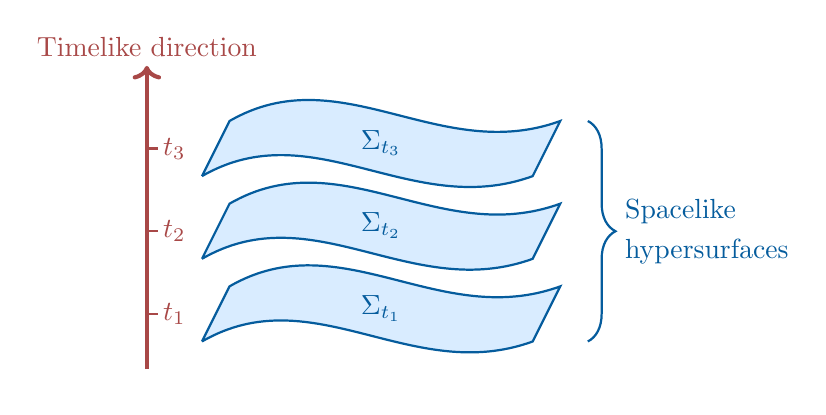
\begin{tikzpicture}[scale=0.7]
    \draw[blue,thick,fill=fau_blue_sk] (-1,0) to[out=30, in=200] (5,0)
         to (5.5,1) to [out=200, in=30] (-0.5,1) to (-1,0);
    \node[blue] at (2.25,0.6) {$\Sigma_{t_1}$};
    \node[rose] at (-1.5,0.5) {$t_1$};
    \draw[thick,rose] (-2,0.5) -- (-1.8,0.5);

    \draw[blue,thick,fill=fau_blue_sk] (-1,1.5) to[out=30, in=200] (5,1.5)
         to (5.5,2.5) to [out=200, in=30] (-0.5,2.5) to (-1,1.5);
    \node[blue] at (2.25,2.1) {$\Sigma_{t_2}$};
    \node[rose] at (-1.5,2) {$t_2$};
    \draw[thick,rose] (-2,2) -- (-1.8,2);

    \draw[blue,thick,fill=fau_blue_sk] (-1,3) to[out=30, in=200] (5,3)
         to (5.5,4) to [out=200, in=30] (-0.5,4) to (-1,3);
    \node[blue] at (2.25,3.6) {$\Sigma_{t_3}$};
    \node[rose] at (-1.5,3.5) {$t_3$};
    \draw[thick,rose] (-2,3.5) -- (-1.8,3.5);

    \draw[line width=1.5,rose,->] (-2,-0.5) to (-2,5);
    \node[rose,above] at (-2,5) {Timelike direction};

    \draw[blue,thick,decorate,decoration={brace,mirror,amplitude=10pt}]
                  (6,0) -- (6,4);
    \node[right,blue,align=left] at (6.5,2) {Spacelike \\ hypersurfaces};
\end{tikzpicture}
\end{minipage}
\hfill
\begin{minipage}{0.38\textwidth}
\centering
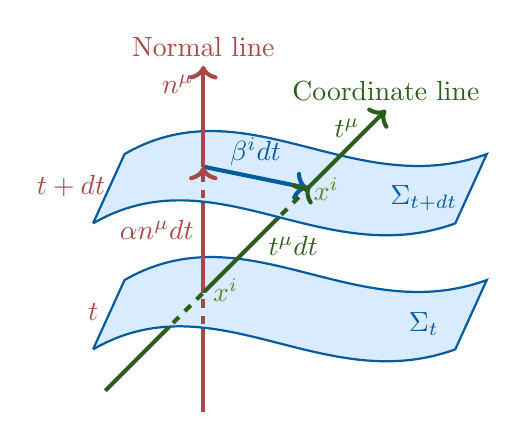
\begin{tikzpicture}[scale=0.8]

    \draw[line width=1.5,forest_green](1,0.9) ++ (-135:0.7) -- ++ (-135:1.5);
    \draw[line width=1.5,rose] (1,-1) to (1,0.36);

    \draw[blue,thick,fill=fau_blue_sk] (-0.75,0) to[out=30, in=200] (5,0)
         to (5.5,1.1) to [out=200, in=30] (-0.25,1.1) to (-0.75,0);
    \node[blue] at (4.5,0.4) {$\Sigma_{t}$};
    \node[rose] at (-0.75,0.6) {$t$};

    \draw[line width=1.5,rose] (1,0.9) to (1,2.36);
    \node[left,rose] at (1,1.9) {$\alpha n^\mu dt$};

    \draw[line width=1.5,forest_green](1,0.9) ++ (45:0.02) -- ++ (45:1.8);

    \draw[blue,thick,fill=fau_blue_sk] (-0.75,2) to[out=30, in=200] (5,2)
         to (5.5,3.1) to [out=200, in=30] (-0.25,3.1) to (-0.75,2);
    \node[blue] at (4.5,2.4) {$\Sigma_{t + dt}$};
    \node[rose] at (-1.1,2.6) {$t + dt$};

    \draw[line width=1.5,blue,->](1,2.9) 
        to node[above,blue] {$\beta^i dt$} (2.66, 2.56);

    \draw[line width=1.5,rose,dashed] (1,0.4) to (1,0.9);
    \draw[line width=1.5,rose,dashed,->] (1,2.4) to (1,2.9);
    \draw[line width=1.5,rose,->] (1,2.9) to (1,4.5);

    \draw[line width=1.5,forest_green,dashed](1,0.9) ++ (-135:0.02)
                                                 -- ++ (-135:0.7);

    \node[green,above right] at (2.6, 2.2) {$x^i$};
    \node[green,above right] at (1,0.6) {$x^i$};

    \draw[line width=1.5,forest_green,dashed,->]
        (1,0.9) ++ (45:1.75) -- ++ (45:0.65);

    \node[right,forest_green] at ($(1,0.9) + (40:1.15)$) {$t^\mu dt$};

    \draw[line width=1.5,forest_green,->]
        (1,0.9) ++ (45:2.35) 
        to node[above,forest_green] {$t^\mu$} ++ (45:1.75);

    \node[forest_green,above] 
        at ($(1,0.9) + (45:2.35) + (45:1.75)$) {Coordinate line};

    \node[rose,left] at (1,4.2) {$n^\mu$};
    \node[rose,above] at (1,4.5) {Normal line};

\end{tikzpicture}

\end{minipage}

\caption{
(a) Spacelike hypersurfaces sliced along the timelike direction. 
(b) Relation between slices showing lapse $\alpha$ and shift $\beta^i$.
}
\end{figure}

By using the orthogonal projection operator to the hypersurface $\perp_{ab} = \delta_{ab} +n_a n_b$ we can project all  the relevant quantities that we require such as the metric, Riemann curvature tensor etc. This projected part of $g_{ab}$ is called spatial metric $\gamma_{ab}$ and D is the derivative associated with this metric. We define extrinsic curvature $K_{ab}$ to be $-\gamma^c_a \nabla_c n_b$ which in vague terms give the information of the time derivative of the spatial metric by the relation $K_{ab} = -\mathcal{L}_n \gamma_{ab}$ where $\mathcal{L}$ is the lie derivative with respect to a vector field. Using all these we can decompose the Einstein's equations into a set of constraint equations and evolution equations as given below.
\begin{equation}
\label{eq:Constraints}
R + K^2 - K_{ab} K^{ab} = 16\pi \rho 
\qquad
D_b K^{ab} - D^a K = 8\pi j^a,
\end{equation}
which correspond to Hamiltonian and momentum constraints respectively, R corresponds to Ricci scalar associated with the $\gamma_{ab}$, $j^a =- \perp T_{ab}n^b, s_{ab}= \perp T_{ab}, \mathcal{\rho} =T_{ab}n^a n^b $ \footnote{$\perp$ means using projection operator on every free index}

\[
\partial_t \gamma_{ij} 
= -2\alpha K_{ij} + \mathcal{L}_{\beta}\gamma_{ij},
\]
\[
\partial_t K_{ij} 
= - D_i D_j \alpha 
  + \alpha( R_{ij} 
  - 2 K_{ik} K^{k}{}_{j} 
  + K K_{ij})
  + 4\pi \alpha \!\left[\, \gamma_{ij}(s - \rho) - 2 s_{ij} \right]
  + \mathcal{L}_{\beta} K_{ij}.\footnote{where i,j $-> $1,2,3 (Spatial)}
\]
 Now we can see that the GR equations have been formulated into a way which is ideal for time evolution using standard PDE techniques(Since all the elements in the RHS are spatial). However, more modern formulations such as BSSN, Z4C, and related systems include constraint-damping mechanisms that improve numerical stability, since in a discretised scheme the constraints cannot be satisfied exactly. It is also well known that the constraint subsystem is closed, meaning that the time derivatives of the constraints depend only on the constraints themselves. Consequently, if the constraint equations are solved initially, they remain satisfied for a finite time during the evolution. For further details, see \cite{hilditch_2024}.

\section{Critical Phenomena in Gravitational Collapse}

\section*{Recap and Motivation}

\section{Horizons}

The main tool we use to classify spacetimes to subcritical or supercritical is by probing to find horizons, specifically Apparent Horizons (AHs) in the evolved slice. The main advantage of AH is that, unlike event horizons they are not \textit{teleological} i.e we dont need the information about the complete spacetime to get the information of apparent horizon. In numerically computed dynamical spacetimes like ours, we might not be in the position to evolve it completely inorder to classify them, hence AHs are the right tool to understand them.

But what is an AH and why does it relate to the notion of a singular spacetime?

Essentially an AH can be defined as the outermost, Marginally Outer Trapped Surface (MOTS) which are smooth closed 2-dimensional submanifold S in the spacetime slice that satisfies the condition that the expansion of the outgoing null geodesics vanishes at each point in S. The expansion is defined as 

$$
\Theta = h^{ab} \nabla_a \zeta_b \qquad \text{where} \; h^{ab}= g^{ab}-s^as^b + n^a n^b 
$$

$h^{ab}$ is the induced metric of the 2-dimensional submanifold, $s^a$ is its normal vector and $\zeta$ is the tangent vector along the outgoing null geodesic . Solving this we get the equation of the form,

\begin{equation}
\Theta = -K + D_i s^i +s^is^j K_{ij} 
\label{Horizon}
\end{equation}

Hence, our aim is to find surfaces satisfying ($\Theta = 0$), and we identify the apparent horizon (AH) as the \textbf{outermost marginally outer trapped surface (MOTS)}.

The importance of apparent horizons is closely tied to the singularity theorems of general relativity. These theorems state that, under suitable energy conditions (such as the \textit{null energy condition}, which is satisfied in vacuum since ($T_{ab}=0$)) and global hyperbolicity (satisfied since the initial data is constraint satisfying), the presence of a trapped surface implies that the spacetime is geodesically incomplete, i.e., contains a singularity.

Thus, the formation of a MOTS or apparent horizon serves as a strong indicator of black hole formation in the spacetime’s future development. This provides a practical and geometric criterion for classifying spacetimes in our analysis.


\section{Gauge Freedom in GR (NR)}

One of the most important characteristic of GR is its so called diffeomorphism invariance which essentially means
that the "physics" inside theory is unchanged under smooth coordinate transformations. In other words, different coordinate systems (or gauges) can describe the same underlying spacetime geometry.


Mathematically, this invariance implies that if $g_{\mu\nu}(x)$ is a solution to Einstein's equations, then so is the transformed metric under a diffeomorphism $x^\mu \rightarrow x'^\mu(x)$, with the metric transforming as
\begin{equation}
g'_{\mu\nu}(x') = \frac{\partial x^\alpha}{\partial x'^\mu} \frac{\partial x^\beta}{\partial x'^\nu} g_{\alpha\beta}(x).
\end{equation}

Often in theoretical studies we utilise various gauges to uncover the internal dynamics of the spacetime variables. The easiest example would in the case of gravitational waves where we often assume a linearised gravity ($g_{\mu\nu}= \eta_{\mu \nu} + h_{\mu \nu}$ where $O(h) << 1$) where the Minkowskian flat space metric is considered as the background metric of the spacetime.  Here to retrieve the notion of gravitational waves we use something known as Lorenz gauge or De Donder gauge ($\partial^{\mu} \bar{h}_{\mu\nu}$) where $\bar{h}$ is the trace reversed metric perturbation. 
Using this gauge we will be able to see that, the metric perturbation has formalised into the form of a wave equation.

$$
\Box \bar{h}^{\mu\nu}= -16 \pi T^{\mu \nu}
$$
This is finest and easiest example of utilising gauges to understand the internal physics. But in the case of the NR, it is utilised differently. As
we know in NR, we try to see Einstein's equations as a set of PDE's to solve numerically. But to solve a problem numerically it is essential that the problem we are solving is \textit{well-posed} and devoid of any coordinate artifacts that coordinate system may evolve into(coordinate singularities , constraint violation and so on). So essentially, we utilise the gauge freedom to counter these problems. Based on how we tackle them has given rise to various formulations of NR like BSSN, Z4C etc. In our case we use the Generalised Harmonic Formulation of NR.

\section{Generalised Harmonic Gauge}

The main advantage of the Generalised Harmonic gauge is that it is, by construction, a well-posed formulation of Einstein's equations. This makes it particularly suitable for numerical evolution, as it provides a strongly hyperbolic system with well-defined characteristic structure. Due to this property, practical considerations aside, in theory they are ideal for any kind of numerical evolutions performed with GR in mind.  The well-posedness of this formulation comes from the trace reversed form of Einstein's equation i.e



\begin{equation}
R_{\mu\nu}
= -\frac{1}{2} g^{\alpha\beta} \partial_\alpha \partial_\beta g_{\mu\nu}
+ \partial_{(\mu} \Gamma_{\nu)}
+ \Gamma^\alpha \Gamma_{\mu\nu\alpha}
- \Gamma^\alpha_{\mu\beta} \Gamma^\beta_{\nu\alpha}
\label{GHG}
\end{equation}

where $
\Gamma^\mu = g^{\alpha\beta} \Gamma^\mu_{\alpha\beta}$ called the contracted Christophel symbols. The well-posedness or ill-posedness of a PDE is often determined by its principal terms (Terms containing the highest derivatives). In our problem, the principal terms are the first and the second part of the Equation \ref{GHG} since they contain the second derivatives of the metric. But since the wave equation is a well posed problem, the problematic part of the equation is the second term (derivative of contracted Christophels). But for that we can utilise the gauge freedom to ensure that they don't contain second derivatives of the metric i.e
$\Gamma^a=\nabla_b \nabla^b x^a=-H^a(x,g)$ where $H^a$ is called the Gauge Source function and it is a function of atmost the metric and not its derivatives.

This gives us the following equations of motion for the lapse($\alpha$) and shift($\beta$)

\begin{equation}
\partial_t \alpha = -\alpha^2 (K + H_n) + \mathcal{L}_\beta \alpha
\qquad \partial_t \beta^i = \alpha^2 (\Gamma^i + \perp H^i) - \alpha D^i \alpha + \beta^j \partial_j \beta^i
\label{lapse=shift}
\end{equation}
where $H^n= n^a H_a$

The $H^a$'s are freely specifiable functions but as we mentioned before, we choose it in a way to have proper evolutions without any coordinate pathologies. That choice will be mentioned in the coming sections.
% Remember to input this to the presentative tex file before compiling.
\chapter{Methodology}

\section{Time Evolutions of Twist-included Brill wave Initial Data}

With the new twist included Brill wave initial data that we constructed, we evolved the initial data in \texttt{BAMPS} NR framework. Unlike the previous tests of Brill waves, we have to evolve the non-diagonal components of the spacetime tensors as well due to the usage of new spatial metric ansatz due to the inclusion of twist. Due to the axisymmetric nature of the problem in hand, we use the cartoon method to simplify the computational costs.

\subsubsection{Cartoon Method \cite{alcubierre_brgmann_holz_takahashi_brandt_seidel_thornburg_2001}}
\label{Cartoon}

In general, performing full 3-D simulations in General Relativity is computationally very expensive due to the dimensionality of the problem. However, when the system possesses axisymmetry, one can exploit this symmetry to significantly reduce computational cost without losing essential physical information.

The cartoon method is a technique that allows one to evolve axisymmetric spacetimes using a reduced computational domain while still employing a Cartesian grid. Instead of evolving the full three-dimensional domain, the evolution is restricted to a thin slab around the symmetry plane (typically the $y=0$ meriodonal plane), consisting of only a few grid points in the symmetry direction.

The key idea is that derivatives in the symmetry direction (e.g., the $y$-direction) can be reconstructed using the assumption of axisymmetry. This is achieved by performing suitable rotations of the evolved variables around the symmetry axis. For a tensor field $T$, its value at off-plane points required for finite difference stencils is obtained by rotating the on-plane data using the Killing symmetry associated with rotations about the axis. Hence essentially our computational domain for the whole problem is the \textbf{Cartesian X-Z} plane.


\subsubsection{Harmonic Damped Wave Gauge (HDWG)}
\label{HDWG}
Harmonic Damped Wave Gauge (HDWG) is obtained by modifying the harmonic gauge condition with a damping term in the gauge source function, turning the coordinate condition into a damped wave equation. This suppresses unphysical gauge modes and stabilizes the coordinate evolution during numerical simulations. The gauge source function for it are

$$
H_a = \mu_L \log \left( \frac{\gamma^p}{\alpha} \right) n_a - \mu_s \alpha^{-1} g_{ai}\beta^i
$$

In black-hole spacetimes, particularly near horizon formation, one often observes a rapid growth of the spatial metric determinant $\gamma$ due to coordinate stretching. The first term in $H_a$, through the logarithmic factor $\log(\gamma^p / \alpha)$, acts to counter this growth by driving a collapse of the lapse $\alpha$, thereby controlling the increase in spatial volume elements. The second term damps the shift vector $\beta^i$, suppressing distortions in the spatial coordinates. For more details, refer \cite{lindblom_szilágyi_2009}

Together, these terms act to control gauge dynamics, preventing the development of large coordinate distortions and stabilizing the evolution near strong-field regions.Since $\mu_L$ and $\mu_s$ sets the time scale where these damping acts, a bit of tuning to find the right parameters are required for proper gauge evolutions which becomes essential in out work.

Using Equation \ref{lapse=shift}, the evolution equation for the lapse and shift becomes, 


\section{Horizon Finding}

In our axisymmetric setting, to locate surfaces satisfying the vanishing expansion condition in Eq.\ref{Horizon}, the problem reduces to a one-dimensional equation in the polar angle, so that the horizon equation becomes an ordinary differential equation. To solve them, we use the \texttt{AHLoc3D} tool which uses a spherical parameterisation for the horizon shape with a parabolic flow method \cite{thornburg_2007}. Essentially, it makes use of guess surfaces in such a way that the outermost MOTS is inside the surface, calculates the expansion at a number of points based on the resolution and the "flows" towards lesser and lesser expansion values based on a pseudo time stepping ($\lambda$), ie
$$
\partial_\lambda x^i = - \Theta s^i
$$
where $s^i$ is the normal vector to the surface.

Additionally in the case of \texttt{AHLoc3D}, the spherical parameterisation used which is $r = F(\theta)$ can only find ray-body/star-shaped horizons. This means that if we draw a ray from the center to the horizon it should only touch horizon once ie the function should not be multivalued in r. This parametrisation begins to break down even before the surface becomes strictly multivalued. In particular, when the surface develops regions where the radial direction becomes tangent to the horizon (i.e., where the outward normal has no radial component), the function $F(\theta)$ develops large gradients or vertical tangents. Numerically, this corresponds to a loss of regularity in the representation, and the horizon finder can fail to converge even though a smooth surface still exists.

Thus, the method is limited not only by true multivaluedness, but also by configurations approaching it, where the surface ceases to be well-described as a function $r(\theta)$.


Despite this limitation, such a parametrisation significantly simplifies the apparent horizon finding problem by reducing it to a one-dimensional equation in $\theta$, making it computationally efficient and straightforward to automate. Consequently, it has become a practical and widely adopted approach in numerical relativity. 
\begin{figure}[!hbt]
    \centering
    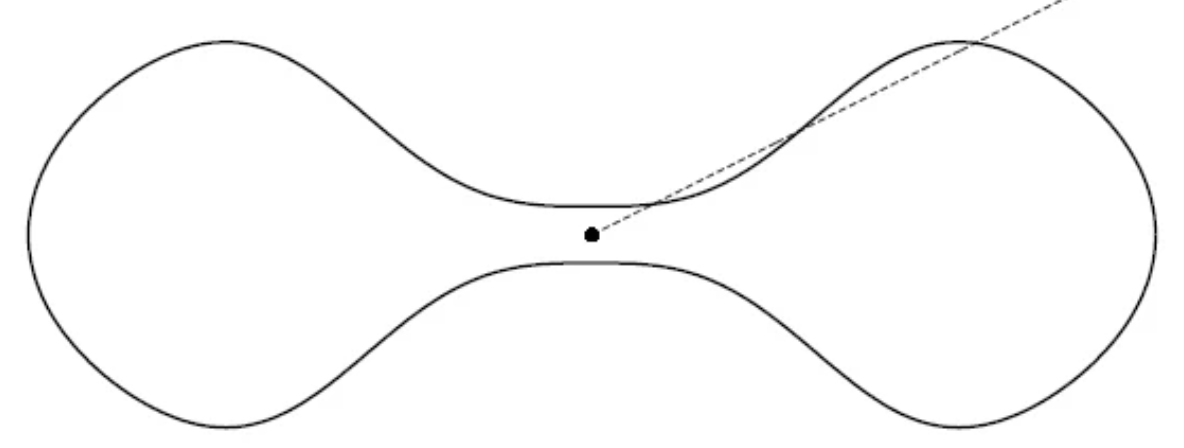
\includegraphics[scale=0.23]{../figures/Screenshot_2026-04-05_14-48-44.png}
    \caption{An example for a non-ray body horizon. Here the r = F($\theta$) parameterisation breaks and \texttt{AHLoc3D} method won't be able find this type of a horizon in the spacetime \cite{thornburg_2007}.}
\end{figure}

Moreover, prior studies of vacuum critical collapse have not indicated the necessity for more general surface representations, as the horizons encountered in those scenarios remain well approximated by star-shaped surfaces. But as we will mention in the coming sections, the inability to tune towards the threshold made us rethink regarding this assumption as a hypothesis which proved to be the correct approach.

We also use a complementary method based on a Cartesian parameterisation with a shooting algorithm, which similarly reduces to solving an ODE in axisymmetry. This removes the ray body limitation that we faced previously but the method uses the Cartoon method as in Sec.\ref{Cartoon} since this search is limited on the y=0 plane and the surface becomes a curve which is parameterised as $X^i (\lambda) = ({X(\lambda),0,Z(\lambda))}$ 

For this method, we integrate the Eq.\ref{Horizon} with this new parameterisation and we get two coupled ODE's of the form in X and Z.

Along the symmetry axis, we begin by making initial guesses for the point at which the horizon intersects the $z$-axis. For each such guess, we integrate the coupled ODEs to obtain a candidate curve $(X(\lambda), Z(\lambda))$. This defines a shooting problem, where we search for solutions that return to the axis, i.e., satisfy $X(\lambda_{\max}) = 0$ for some $\lambda_{\max} > 0$.

In addition to this closure condition, regularity at the axis requires the tangent vector to be aligned with the radial direction in the meridional plane, which imposes the boundary condition $u^z(\lambda_{\max}) = 0$. We therefore select those curves that both return to the axis and satisfy this smoothness condition.

Finally, these candidate solutions are passed to a root-finding algorithm such as \texttt{BRENTQ} to determine the precise initial condition that yields a closed and smooth horizon. For further details, see~\cite{khirnov_2022}.



% Remember to input this to the presentative tex file before compiling.
\chapter{Observations,Results and Challenges}

Critical phenomena in gravitational collapse are most clearly understood in spherical symmetry, where the approach to the critical regime is comparatively straightforward. In this case, the field equations reduce to a system of coupled one-dimensional partial differential equations, which can be solved with relatively high numerical accuracy. Indeed, in the pioneering work of Matthew Choptuik \cite{choptuik_1993}, the critical parameter was tuned to nearly machine precision, reaching approximately 15 decimal places.

However, once symmetry assumptions are relaxed, the problem becomes significantly more challenging. In the literature, studies of axisymmetric vacuum collapse typically achieve only about 5–7 digits of precision in tuning the critical parameter. This limitation arises both from the increased computational difficulty of solving multidimensional partial differential equations and from the intrinsic nature of critical phenomena, which involve the development of increasingly fine spatial and temporal structures near the threshold of black hole formation.

For the family of initial data considered in this work, the best-tuned critical parameter is found to be $(p^* = 4.110 \pm 0.003)$. Despite this comparatively modest level of tuning, we are able to extract a critical exponent of approximately $( \gamma \approx 0.55 \pm 0.32 )$, demonstrating the robustness of the scaling behaviour even without extremely fine-tuned initial data.

The quoted uncertainty in the critical parameter arises from the inability to unambiguously distinguish between subcritical and supercritical evolution within this narrow region of parameter space. In particular, near the threshold, small variations in the parameter lead to qualitatively different outcomes, and within our numerical resolution this transition cannot be resolved more precisely. This limitation propagates into the determination of the scaling exponent, contributing to the relatively large uncertainty in ($\gamma$).
\begin{figure}[!hbt]
    \centering
    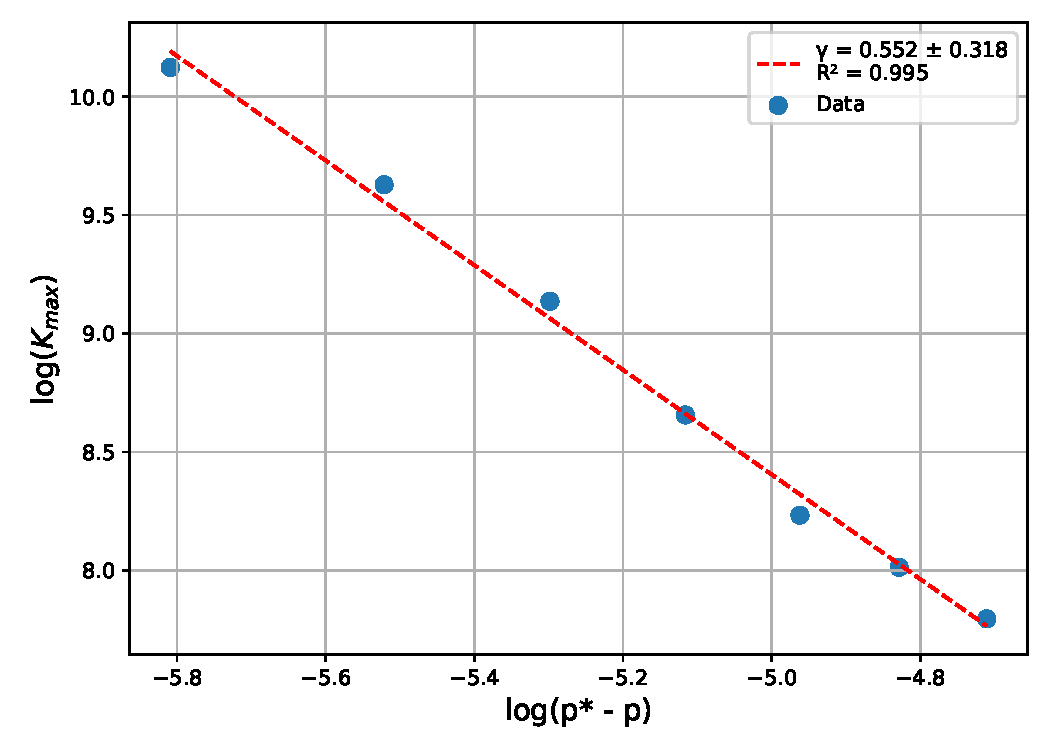
\includegraphics[scale=0.6]{../notebooks/plusfamily.pdf}
    \caption{Log--log plot of the maximum Kretschmann scalar $K_{\max}$ in subcritical evolutions as a function of $(p^* - p)$. Each data point corresponds to an independent simulation, with typical computational cost of $\sim 4000$ core-hours per run. The approximate linear behaviour supports the expected power-law scaling $K_{\max} \sim (p^* - p)^{-4\gamma}$ near criticality.}
\end{figure}

For the current family that we have chosen, we see a $R^2$ goodness of fit value of 0.995 which gives an additional assurance that there indeed exists some linear scaling even at this level of tuning.



But in this regard, more work needs to be done to tune more into the critical regime and investigate the critical phenomena (Presence of self-similiar structures and so on).

For example, as the parameter is tuned closer to the critical value, the evolution exhibits increasingly pronounced oscillatory features in the curvature, suggestive of the onset of echoing behaviour. These structures appear as repeated, self-similar peaks in the Kretschmann scalar as a function of proper time. However, due to the limited level of tuning and numerical resolution in the present simulations, these features cannot be conclusively identified as true discrete self-similarity. Achieving a more definitive verification would require finer tuning of the critical parameter and higher resolution to resolve the increasingly small spacetime scales involved.

\begin{figure}[!!hbt]
    \centering
    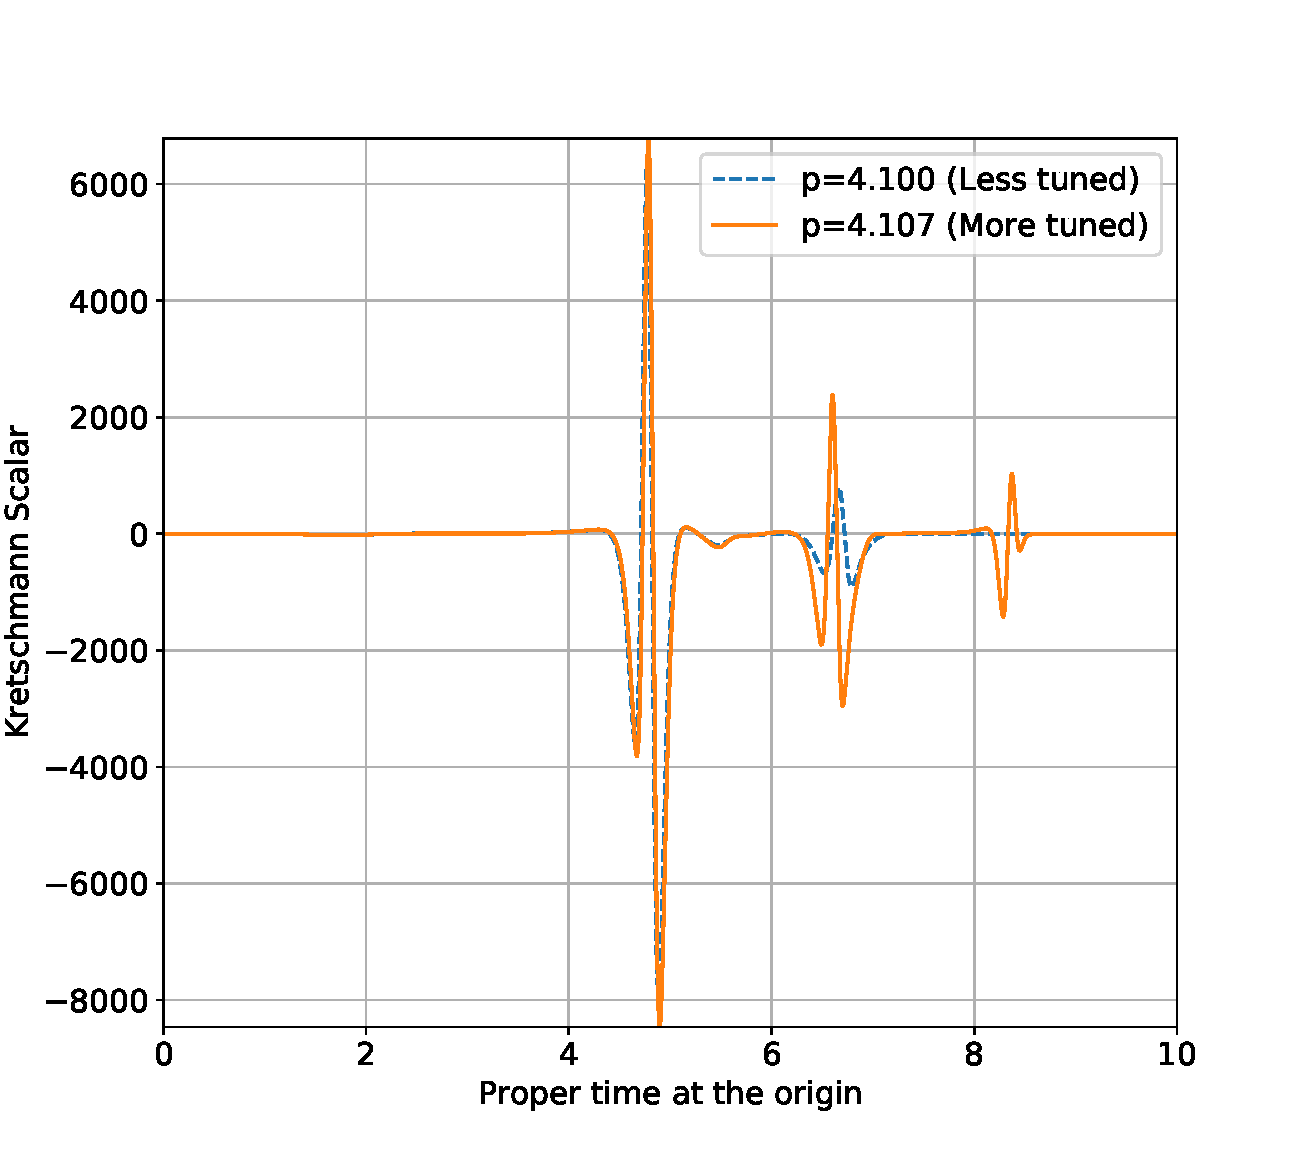
\includegraphics[scale=0.6]{../figures/feature.pdf}
    \caption{Log--log plot of the maximum Kretschmann scalar $K_{\max}$ in subcritical evolutions as a function of $(p^* - p)$. Each data point corresponds to an independent simulation, with typical computational cost of $\sim 4000$ core-hours per run. The approximate linear behaviour supports the expected power-law scaling $K_{\max} \sim (p^* - p)^{-4\gamma}$ near criticality.}
    \label{feature}
\end{figure}


\textbf{But what makes tuning and classifying spacetimes difficult?}

As the critical threshold is approached, it becomes increasingly difficult to classify a given evolution as subcritical or supercritical. In particular, near-critical evolutions may:

\begin{enumerate}
\item not exhibit clear dispersal of curvature to spatial infinity,
\item not form an apparent horizon detectable by standard horizon-finding tools,
\end{enumerate}

thereby making the outcome ambiguous within finite numerical resolution. This could be attributed to certain reasons as to why.

\section*{Development of Coordinate Pathologies}



\subsection*{Courant Condition and Resolution Limits}

As we approach the critical regime, the solution develops structure on increasingly small spatio-temporal scales. This imposes a fundamental restriction on the timestep through the Courant – Friedrichs – Lewy (CFL) condition, which is required for the stability of explicit numerical schemes.

The Courant condition states that the numerical domain of dependence must include the physical domain of dependence. For a hyperbolic system with characteristic speed $v_{\max}$, this leads to the condition
\[
\Delta t \leq C \frac{\Delta x}{v_{\max}},
\]
where $C < 1$ is the Courant factor determined by the numerical scheme.

This condition has important consequences near criticality. To resolve the features \texttt{BAMPS} uses Adaptive Mesh Refinement (AMR) which adjusts the spatial grid sizes to capture the dynamics that happen in smaller and smaller scales. As finer spatial resolution ($\Delta x \to 0$) is required to resolve the small-scale features that emerge, the timestep must also decrease proportionally. Consequently, the computational cost increases significantly, since the number of timesteps required scales inversely with $\Delta t$. With our current computational resources we were only able to tune to about 3 decimal places due to that reason.

Additionally, the dynamics of critical phenomenon is in such a way as we tune towards the threshold of collapse, the evolution resembles each other to even more duration of evolution until the solution "chooses" an end point, be it a singular spacetime or dispersion. So essentially we will have to evolve more as we tune the parameter more to reach the critical regime.



Therefore, the combination of shrinking physical scales and the CFL constraint severely limits how close one can tune to the critical parameter in multidimensional simulations. This is one of the primary reasons why achieving high precision in non-symmetric critical collapse is significantly more challenging than in spherical symmetry.





\begin{figure}
    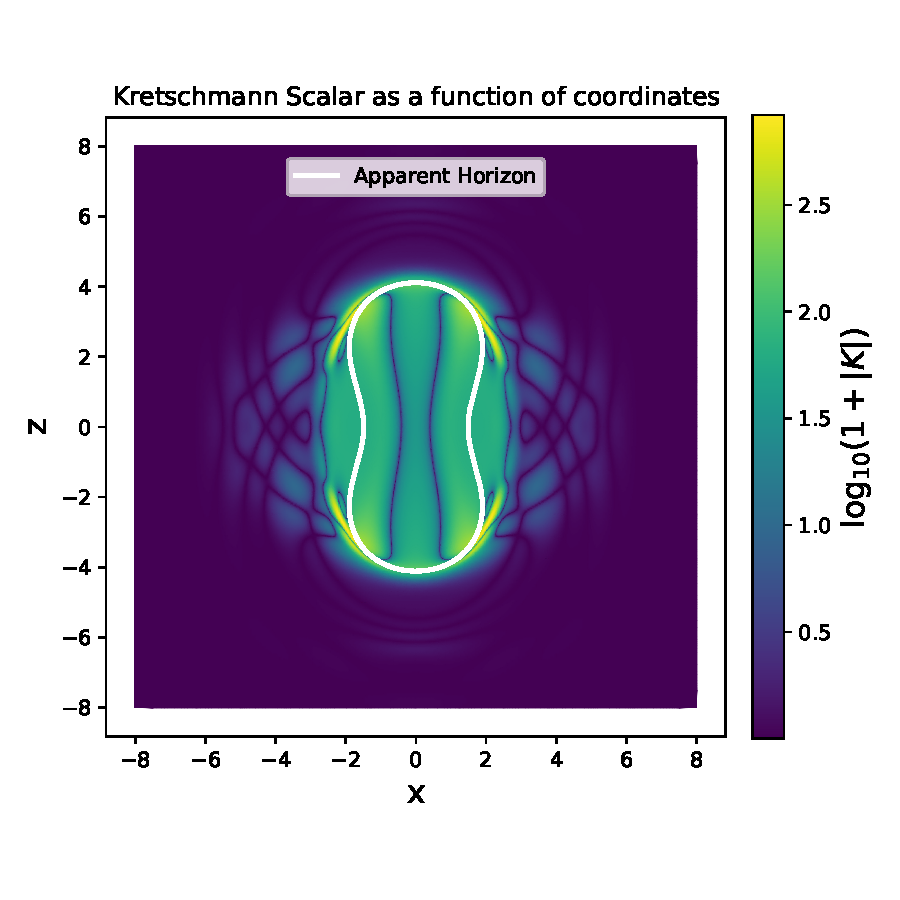
\includegraphics[scale=0.8]{../notebooks/figure.pdf}
    \caption{}
\end{figure}

\subsubsection{Harmonic Horizon Marching Gauge}
\label{HHMG}
Since GR has an intrinsic gauge freedom built into it, it will be reflected when we do simulations using NR as well. Hence we will have to choose a gauge but in the case of simulations they are chosen by the stability it confers to the simulations.

In \texttt{BAMPS}, the usual gauge that we use is HDWG (Harmonic Gauge). Here the evolution equations for the lapse becomes,

\[
\mathcal{L}_n \log \alpha = - (H_n +K)
\]

where $H_n$ is the free choosable function which only contains the metric and not its derivatives.

Inorder the push the lapse to 1 we add an extra term into the harmonic function in such a way that it adds a term $\eta_{hm}(\alpha-1)$ into the evolution equation for lapse

\[
\partial_t \alpha -\beta^i \partial_i \alpha= -\alpha^2(H_n + K)
\]

The extra term that in $H_n$ is $\eta_{hm} \alpha^{-2} (\alpha-1)$

\[
\partial_t \alpha -\beta^i \partial_i \alpha= -(\eta_{hm} (\alpha-1) + \alpha^2 K)
\]

So in $H_a$ an extra term of $-\eta_{hm} \alpha^{-2} (\alpha - 1) n_a$ is added

So New $H_0=.... + \eta_{hm} \alpha^{-1} (\alpha-1)$

\[
\partial_t H_0 = +\eta_{hm} \alpha^{-2} \partial_t \alpha
\]

\[
\partial_i H_0 = +\eta_{hm} \alpha^{-2} \partial_i \alpha
\]
\chapter{Conclusion and Future directions}
In this work, we have investigated critical phenomena in axisymmetric vacuum spacetimes using Brill wave initial data with twist. Through the construction and evolution of one-parameter families of initial data, we identified a threshold separating dispersion from black hole formation. For the family of pure twisting Brill waves constructed here, the critical parameter has been tuned to a precision of three decimal places. 
While previous studies typically achieve higher precision (of order $\sim 6$ decimal places), the present level of tuning corresponds to an intermediate stage in the approach to the critical threshold. Nevertheless, it already allows us to observe a scaling relation between the maximum of the Kretschmann scalar and the distance from the critical parameter. An estimate of the critical exponent can also be obtained from this scaling behaviour. However, given the current level of tuning, these results should be regarded as preliminary, and further refinement is required before drawing more definitive conclusions.

Additionally, near-critical evolutions exhibit echo-like features in the curvature, suggestive of underlying self-similar dynamics. While the current level of tuning and resolution does not allow for a definitive identification of discrete self-similarity, these results are consistent with expectations from critical collapse. 

We have also discussed the numerical challenges encountered in this work and possible strategies to mitigate them. In particular, the use of a Cartesian-based apparent horizon finder has already improved the exploration of the parameter space and is expected to facilitate further tuning toward the critical regime.
The substantial computational cost ( $\approx$4000 core-hours per simulation) further highlights the difficulty of accessing the critical regime in less symmetric spacetimes.

\section*{Future Directions}
An immediate direction for future work is to achieve higher precision in tuning the critical parameter. This would enable more accurate determination of critical exponents and a clearer assessment of universality. Exploring multiple families of initial data will be essential to establish whether the observed behaviour is truly universal. Until now, we have only tried pure twisting Brill wave i.e. Seed function $q(\rho,z) =0 $ and after trying different families in that, we will move on to adding the influence of the seed function along with twist variables. Then an even stronger test would be to take the other class of axisymmetric vacuum initial data which are Teukolsky waves, modify them to include twist and conduct similar tests in that data. We expect that to be easier with the insights that we have gained with this experiment.

A much deeper investigation of self-similarity is also required. Higher resolution simulations may allow for the extraction of echoing structure and scaling periods, providing stronger evidence for the nature of the critical solution.

Understanding the role of twist remains an open problem. In particular, it is important to determine whether twist gives rise to new classes of critical solutions or modifies existing ones. This could provide insight into the broader structure of the solution space in axisymmetric vacuum spacetimes.

From a numerical perspective, improving gauge choices and developing more robust horizon-finding techniques will be crucial. We have already implemented a new gauge choice that appears to facilitate reaching the horizon more efficiently; however, it is not discussed here, as it requires further testing and validation. 
Additionally, the Cartesian-based apparent horizon finder currently requires a substantial amount of manual intervention. Developing automated or more robust horizon-finding methods will therefore be an important direction for future work.



% Note:
% Use sections/subsections to structure content within each chapter.

%=========================================================================================
% APPENDICES
%=========================================================================================

%\appendix
%\addappheadtotoc
%%~~~~~~~~~~~~~~~~~~~~~~~~~~~~~~~~~~~~~~~~~~~~~~~~~~~~~~~~~~~~~~~~~~~~~~~~~~~~~~~~~~~~~~~~~%
%                                    APPENDIX TEMPLATE                                    %
%~~~~~~~~~~~~~~~~~~~~~~~~~~~~~~~~~~~~~~~~~~~~~~~~~~~~~~~~~~~~~~~~~~~~~~~~~~~~~~~~~~~~~~~~~%

% Use these after the \appendix command at the end of report.tex
% Appendices work similar to a chapter and are used to provide supplementary information that typically do not contribute to the final page count of a report.

\chapter{Long Appendix Title Here} % Main appendix title

\label{AppendixA} % for referencing this appendix elsewhere, use \ref{AppendixA}

% This is for the header on each page if in use - input a shortened title due to constrictions.
% \lhead{Appendix A. \emph{Short App. Title Here}}

Write your Appendix content here. Sections and subsections can be used as well.
\section{First Appendix Section}
\subsection{First Appendix Subsection}
\subsubsection{First Appendix Subsubsection}
Appendices will show up in the ToC numbered as letters. This is of course totally customizable, please refer to the CTAN documentation (\url{https://ctan.org/pkg/appendix?lang=en}) for further clarity on the same.

%=========================================================================================
% BIBLIOGRAPHY
%=========================================================================================
                             % Include all entries from ref.bib

                             \renewcommand*{\bibfont}{\fontsize{11pt}{12pt}\selectfont}
\setlength\bibitemsep{0.5pt}
\vspace{35pt}
% Start two columns for bibliography ONLY
\begin{multicols}{2}
\setlength{\columnsep}{10pt}   % default ~15pt
\printbibliography[heading=bibintoc]
\end{multicols}
     % Bibliography in ToC

\end{document}